
%\addcontentsline{toc}{section}{Introduction} % Ajout dans la table des matières
\section{Résumé} 

Pendant ces quatre mois de stage, notre groupe de recherche travaille avec les employés de \textsc{cmcc} ( China Mobile Communications Corporation ) . L'objectif du sujet est: utiliser les techniques de Fouille de données, étudier les données fournies par le CMCC, et trouver les relations entre les données et les défauts du système 4G. Nous avons fait plusieurs tentatives pour trouver les résultats, et on a utilisé de différents logiciels, j'ai utilisé le R, et mon collègue utilisé Mathlab, nous avons utilisé plusieurs algorithmes (Clusterring, PCA, Association rules, Ajustement). Mais à la fin,  nous avons trouvé qu'à cause des défaut dans la système d'acquisition, les données ne sont pas correct, et nous ne pouvons pas trouver le résultat comme prévu. Mais les recherches que nous avons fait peuvent faire savoir comment utiliser les technique de fouille de données dans le domaine de télécommunication.

\section{Introduction} 
 
Le 3 avril 1973, M. Mation \textsc{cooper} le directeur général de la division communication de Motorola, a effectué un appel téléphonique à Joel \textsc{engel}, son rival et néanmoins confrère chez \textsf{Belle Labs}. c'est le premier appel téléphonique en extérieur, L'idée du téléphone portable devient une réalité. 

Depuis ce jour, la technique développe très rapidement. Pendant les 20 dernières années, il y a déjà quatre générations des standards pour le téléphonie mobile, non seulement nous pouvons appeler les autres, les nouvelles technologies et les Smart-phones nous permettons aussi d'envoyer les messages, de surfer sur l'Internet, d'utiliser le service RTSP(Real Timide Streaming Protocol), et le service VoIP (Voice over Internet Protocole),etc.. Les services de communication téléphonique sont devenus un outil très important dans notre vie.
 
 \subsection{Introduction du CMCC}
 
Fondé en 3 septembre 1997, après le regroupement d'opérateurs des télécommunications en 2008, \textsc{China Mobile Communications Corporation} (\textsf{CMCC})\ref{Fig.sub.1} est devenu un des trois opérateurs des télécommunications en Chine (deux autres sont \textsf{China Unicom Co., Ltd.} et \textsf{China Telecom}). Après plusieurs années de développement, il a construit le plus grand réseau de communications mobiles dans le monde, possède la plus grande base d'utilisateurs dans le monde\ref{Fig.sub.2}. En 2013, le CMCC a 767 million utilisateurs, 630,2 billion \textyen \qquad de revenu, 121,7 billions \textyen de revenus net, et un effectif de 197,030 personnes.
\begin{figure}[H]
	\flushleft
	\subfigure[Logo de China Mobile]{
		\label{Fig.sub.1}
		
\includegraphics[width=1.8in]{images/China_Mobile_2013.png}}\hfill
	\hspace{1in}
%\flushright
	\subfigure[Reseau télécommunication]{
		\label{Fig.sub.2}
		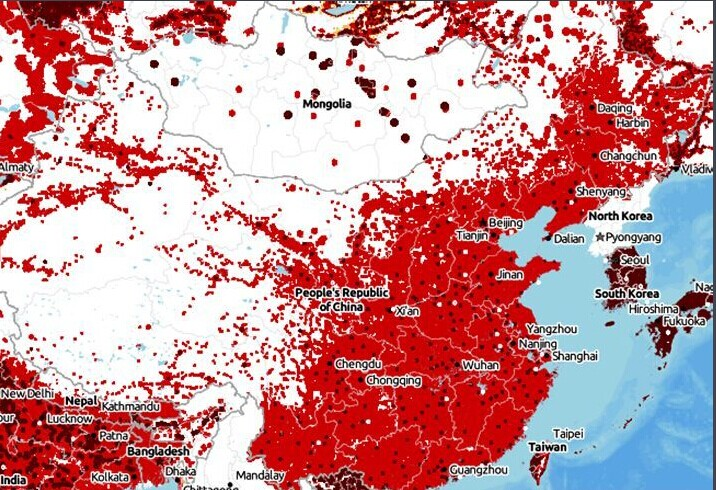
\includegraphics[width=2.0in]{images/reseau.jpg}}
	\caption{CMCC} 
\end{figure}

\subsection{La crise du CMCC}
\subsubsection{La demande de mise à niveau du réseau}
Mais en même temps, le taux de croissance des nouveaux utilisateurs décline de 22,5 \% (2006) à moins de 5\% en 2013 \ref{tauxdecroissance}. Et pour les trois premières mois, bien que l'entreprise soit une fois considéré comme la plus rentable de Chine, le taux de croissance des revenu net n'est que 0,3\%.

      \begin{figure}[H]
          \centering
          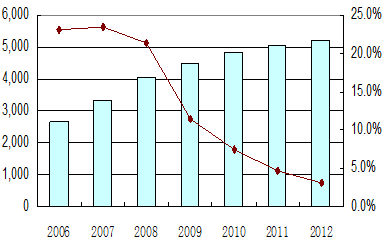
\includegraphics[width=3in]{images/1.png}
          \caption{le taux de croissance est décliner}
          \label{tauxdecroissance}
      \end{figure}
Opérateur des télécommunications Vodafone a fait une étude après qu'il a déployé un réseau 3G(\textsf{the third generation of mobile phone mobile communication technology standards}). Comme le réseau 3G permet des débits (de 2 à 42 Mb/s définis par la dernière génération des réseaux) qui sont bien plus rapides que la génération précédente, par exemple le GSM. Les utilisateurs utilisent bien plus souvent le service internet\ref{vodafone1}. Comme ils utilisent plus du service internet, le data ARPU (Average Revenue Per User) augmente, mais le voix ARPU décline plus rapidement que l'augmentation de data ARPU\ref{vodafone2}. 
 \begin{figure}[H]
 	\flushleft
 	 	\subfigure[Downlink Data Traffic in 2G/3G Network]{
 	 	\label{vodafone1}
 	 	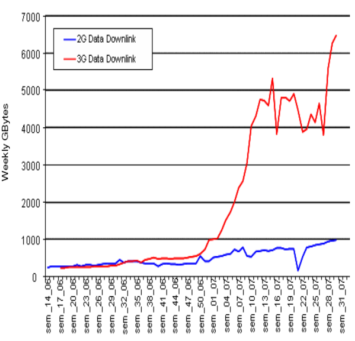
\includegraphics[width=2.0in]{images/4.png}}\hfill
 	\hspace{1in}	 
 	\subfigure[étude de Vodafone]{
 		\label{vodafone2}
 		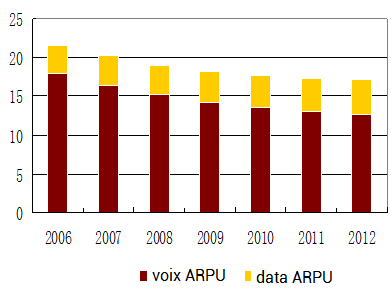
\includegraphics[width=1.8in]{images/2.png}}
 	\caption{Vodafone} 
 \end{figure}
 
Mais l'étude d'Orange nous montre que si nous pouvons fournir des nouvelles technologies qui ont plus haute débit, les utilisateurs utiliseront plus souvent le service data.  \ref{traficparpersonne}
  \begin{figure}[H]
   \centering
   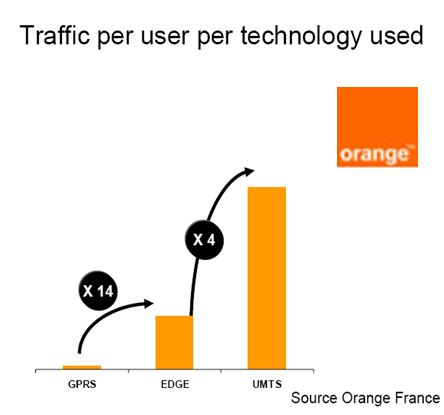
\includegraphics[width=3in]{images/orange.JPG}
   \caption{trafic par personne }
   \label{traficparpersonne}
  \end{figure}
 Des études nous montrent que de nouvelles technologies (comme LTE) peuvent diminuer le prix de revient qui peut assurer le profit de l'opérateur. Mais déployer les nouveaux matériels coute cher, en 2009, le CMCC a dépensé 30 billions \textyen pour construire les stations de réseau 3G, et en 2014, le CMCC a construit 1,5 million stations, à la fin de cette année, il y aura 1,8 million stations, parmi ces station, il y aura 500 mille stations TD-LTE. En ajoutant des équipements 4G, il peut être mis à niveau une station de 3G à 4G. Donc déployer le réseau 4G n'est pas trop cher, selon l'expérience précédente (de 2G à 3G), les utilisateurs vont utiliser plus le service internet, qui peut assurer le profit de l'entreprise.
      \begin{figure}[H]
          \centering
          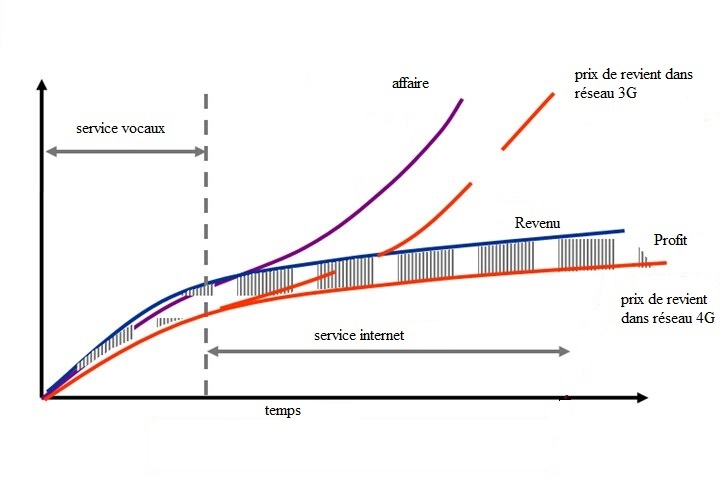
\includegraphics[width=3in]{images/why4G.jpg}
          \caption{4G est plus rentable}
          \label{why4G}
      \end{figure}
      
 \subsubsection{Les changements des moyennes de revenu}
Avant la popularité des téléphones intelligents, et avant la popularité du réseau 3G, beaucoup des utilisateurs du CMCC utilisent le services message pour recevoir des informations comme es nouvelles, les météo, etc. Ces services étaient un moyen de revenu très important pour le CMCC.  Mais maintenant, avec la popularité du smartphone et l'évolution du réseau, les gens peuvent trouver tout les informations sur l'internet. En la vacance du nouvel an chinois 2013, $31,3$ milliards SMS a été envoyé, comparé à cette année, le nombre est $18,2$ milliards SMS, il a réduit $42\%$. Ces informations sont très inquiétantes pour le CMCC.

En conclure, CMCC devez mettre à jour son réseau de télécommunication, mais le mise à niveau du réseau à une réduction de revenu des autres services. Alors CMCC veut apprendre les entreprise comme \textsf{Tencent} et trouver des moyens pour augmenter le revenu.
  \subsection{L'optimisation du réseau}
En plus de l'évolution des technologies, un grand enjeu pour les opérateurs est: l'optimisation du réseau télécommunication. Le réseau de communication mobile est très dynamique, la répartition de la densité du trafic est inégale, fréquence très limitée, etc. La configuration du réseau était toujours sous-optimale, et la perception de l'utilisateur n'est pas très bien. Donc tous les opérateurs doivent toujours reconfigurer/optimiser/maintenir les paramètre du réseau.
  
Les opérateurs peuvent percevoir les données sur Internet, et utilisent ces informations pour trouver les défauts du système, ce peut aider l'entreprise optimiser le système.

Mais l'optimisation du réseau télécommunication est difficile, parce-que les technologies d'optimisation de réseau concerné à savoir la technologie de commutation, la technologie sans fil, la configuration et commutation de la fréquence, la signalisation système, l'analyse de trafic, etc. sont des travaux difficiles, qui exigent une meilleure aptitude des employés.  

Actuellement, l'optimisation du réseau dépend principalement de l'expérience du personnel. Mais des fois, les expériences ne sont pas correctes. Par exemple, si l'entreprise a besoin de savoir le congestionné d'une station, il faut envoyer les employés avec des équipements pendant les périodes de pointe, mais on ne sait pas si les résultats sont corrects \ref{meseau}.  En outre, souvent un seul type de donnée est utilisé pour l'analyse et la comparaison pour optimiser les réseaux, il faut mieux de trouver une solution d'optimisation basée sur toutes les données liées au réseau (telles que les données statistiques de trafic, les données d'essai, etc). Et en raison de l'énorme quantité de données, c'est difficile de traiter en temps opportun. Il est évident que cette méthode est défectueuse. Les défauts du système provoquent la non satisfaction des utilisateurs, ce qui a conduit les défaurs à se multiplier.
      \begin{figure}[H]
          \centering
          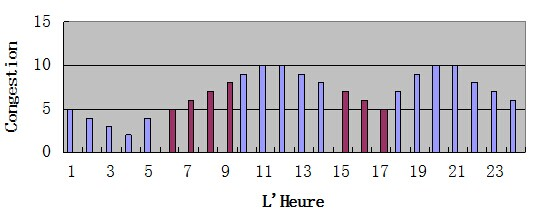
\includegraphics[width=3in]{images/meseau.jpg}
          \caption{Mesure la congestionné d'un station}
          \label{meseau}
      \end{figure}
      
Face à des problèmes complexes, les grandes entreprises commencent à utiliser les techniques de Fouille de données. Cette technique peut aider l'entreprise à prendre faire les décisions plus vite et plus précises.

De ce faire, en Juillet 2013, le CMCC a lancé ce projet avec quatre laboratoires dans trois universités, ils sont
 \href{http://www.tsinghua.edu.cn/publish/newthuen/index.html}{Tsinghua University}, \href{http://en.sdu.edu.cn/}{Shandong University} et \href{http://www.oice.uestc.edu.cn/en/}{University of Electronic Science and Technology of China}. Le projet inclut trois partiel: Fouille de données, gestion du Clound plateforme et modélisation de l'information dans le système.
 

  \subsection{Introduction du laboratoire}
 De 20 Avril 2014 à 20 Juillet 2014, je fait mon stage chez \href{http://203.91.121.76/joomla/}{laboratoire of Next Generation Network Technology \& Application} \textsf{(NGN)} \ref{Logo NGN}. C'est d'un subordonné de \href{http://www.ee.tsinghua.edu.cn/publish/eeen/3776/index.html}{Research Institute of Network And Human-Machine Speech Comunication}, Département Ingénierie électronique, Tsinghua University. Le laboratoire se trouve dans le ROHM bâtiment.
  \begin{figure}[H]
      \centering
      
\includegraphics[width=3in]{images/NGN.jpg}
      \caption{Logo NGN}
      \label{Logo NGN}
  \end{figure}
Les principaux axes de recherche sont Théorie des réseaux, Architecture de l'Internet, Traitement de l'information Internet, recherche dans le domaine de la sécurité Internet, Sentiment analyse, Information hiding, etc.

 Mon tuteur professionnel est \href{http://203.91.121.76/joomla/index.php/staff/teacher/83-huangyongfeng}{M. Yongfeng \textsc{huang}}, vice-directeur du laboratoire NGN. Dans le laboratoire, il y a cinq groupes, chaque groupe a un docteur et son sujet. dans notre groupe, il y a quatre personnes, un étudiant de doctorat de la première année, un étudiant de M1, et une étudiante de Licence de la troisième année et moi. On utilise R et Rstudio, et Hadoop aussi.
 
 \subsection{Objectif du projet}
Dans cet article, nous allons d'abord présenter le réseau de communication mobile, ensuite décrire l'état de l'optimisation du réseau et les techniques pour l'optimisé. pour enfin je présenter notre solution et le conclusion de ce stage.